% !TEX TS-program = XeLaTeX
% !TeX spellcheck = en_US
% !TeX program = xelatex


\documentclass[a4paper, 12pt, titlepage, headsepline, listof = totoc, bibliography = totoc, numbers = noenddot]{scrbook} %
\usepackage[left = 2cm, right = 2cm, top = 3cm, bottom = 3cm]{geometry} % spaces on the sides of the paper
%\usepackage[utf8]{inputenc} %pdflatex
\usepackage{polyglossia} %xelatex
\setdefaultlanguage[variant=british]{english} %xelatex

% fonts and layout (xelatex)
%\defaultfontfeatures{Mapping=tex-text}
\setmainfont[Mapping=tex-text]{Adobe Garamond}
\setsansfont[Mapping=tex-text]{Meta}
\setmonofont{Source Code Pro}
\linespread{1.3}
\frenchspacing
\usepackage{setspace}
\usepackage{microtype}
\usepackage{xspace}
\usepackage{enumitem}
\raggedbottom
\setlist[itemize]{noitemsep, topsep=0pt}

% Graphics, subfigures, and colours
\usepackage{graphicx}
\usepackage[bf,IT]{subfigure}% http://ctan.org/pkg/subfigure
\usepackage{tikz}
\usetikzlibrary{calc,positioning,shadows,arrows,shapes}
%\usetikzlibrary{calc,fit,shapes,shapes.callouts,shapes.symbols,positioning,shadows,arrows,decorations,backgrounds,plotmarks,external}
%\tikzexternalize[prefix=tikz/]

% Listings
\usepackage{listings}

\lstdefinelanguage{MD2}{
  morekeywords={WorkflowElement,WorkflowElements, fires, start, App, startable, appName, package, entity, string,
  date, float, enum, integer, boolean, time, datetime, GridLayoutPane, FlowLayoutPane, TabbedPane, TextInput,
  label, tooltip, type, default, timestamp, OptionInput, options, CheckBox, checked, Label, text, style, Tooltip,
  Button, Image, height, width, src, Spacer, AutoGenerator, exclude, only, textProposition, contentProvider,
  ContentProvider, EntitySelector, color, fontSize, textStyle, main, appVersion, modelVersion, workflowManager,
  defaultConnection, CustomAction, CombinedAction, CustomCodeFragement, SimpleAction, WebServiceCallAction, WebServiceCall, externalWebService, url, method, GET, POST, PUT, DELETE, queryparams, bodyparams, on, from, Container, Content,
  GlobalEventType, OnConditionEvent, elementEventType, GotoViewAction, Workflow, WorkflowStep, ContentProvider, use,
  for, to, latitude, longitude, altitude, citystreet, number, postalCode, country, province, ElementEventType, event,
  valid, empty, filled, and, equals, not, is, or, Condition, Boolean, bind, unbind, Validator, ContainerElement,
  ContentElement, validator, IsIntValidator, NotNullValidator, IsNumberValidator, IsDateValidator, RegExValidator,
  NumberRangeValidator, StringRangeValidator, map, unmap, call, actions, message, min, max, regEx, format, minLength,
  maxLength, RemoteValidator, connection, model, attributes, workflow, ProcessChainStep,step, view, forwardCondition,
  forwardMessage, backwardMessage, backwardCondition, forwardOnEvent, backwardOnEvent, forwardEvents, subProcessChain,
  remoteConnection, uri, ProcessChain, end, defaultProcessChain, onInit, FireEvent, ProcessChainProceed, ProcessChainReverse, ProcessChainGoto, SetProcessChain, GotoView, where, Location, Disable, Enable, DisplayMessage, ContentProviderOperation, ContentProviderReset, inputs, outputs, cityInput, streetInput, streetNumberInput, postalInput, countryInput,FileUpload, UploadedImageOutput, imgHeight,imgWidth,fileUploadConnection, storagePath, file, optional,
  latitudeOutput, longitudeOutput, name, description, proceed, reverse, goto, return, given, do, returnTo, disabled,
  action, if, else, set, elseif},
  otherkeywords={},
  sensitive=true,
  morecomment=[l]{//},
  morecomment=[n]{/*}{*/},
  morestring=[b]",
  morestring=[b]',
  morestring=[b]"""
}
\lstset{
  language=MD2,
  aboveskip=3mm,
  belowskip=3mm,
  showstringspaces=false,
  columns=flexible,
  basicstyle={\footnotesize\ttfamily},
  numbers=none,
  numberstyle=\tiny\color{gray},
  keywordstyle=\color{mauve},
  commentstyle=\color{dkgreen},
  stringstyle=\color{blue},
  breaklines=true,
  breakatwhitespace=true
  tabsize=3
}


%\usepackage{caption} 
\renewcommand{\thesubfigure}{\alph{subfigure}}% (a) -> a
%\usepackage[table]{xcolor}
\definecolor{Lightgray}{gray}{0.9}
\definecolor{dkgreen}{rgb}{0,0.6,0}
\definecolor{gray}{rgb}{0.5,0.5,0.5}
\definecolor{mauve}{RGB}{127,0,85}

% Define ERCIS colors (see official corporate design manual)
\definecolor{ercisblack}{RGB}{0,0,0}
\definecolor{ercisgrey}{RGB}{94,94,93}
\definecolor{ercisred}{RGB}{133,35,57}
\definecolor{ercislightred}{RGB}{200,156,166}
\definecolor{ercisblue}{RGB}{135,151,163}
\definecolor{ercisclaim}{named}{ercislightred}

% Additional ERCIS colors
\definecolor{ercisdarkblue}{RGB}{67,92,139}
\definecolor{erciscyan}{RGB}{0,156,179}
\definecolor{ercisorange}{RGB}{231,124,18}
\definecolor{ercisgreen}{RGB}{135,191,42}

% Define WWU colors (see official Corporate Design manual, p. 21)
\definecolor{pantoneblack7}{RGB}{62,62,59}

%maths
\usepackage{amssymb}
\usepackage{amsfonts}
\usepackage{amsmath}


%STOP ROMAN NUMBERS FROM GROWING TO THE RIGHT IN TAB OF FIGURES!!!!!!11
\makeatletter \def\@pnumwidth{3em}\makeatother 


% notes, reminder
\setlength{\marginparwidth}{1.5cm} % width of todo note
\usepackage[ngerman,textwidth=1\marginparwidth,textsize=scriptsize,backgroundcolor=yellow,linecolor=blue]{todonotes} %,disable
%\reversemarginpar % put todo note left, where the margin is (way) larger (disabled, since it's not)

%Acronyms
%\usepackage[printonlyused]{acronym}

%Quotations
\usepackage{csquotes}
\setquotestyle[american]{english}

% References Section
%\usepackage[backend=biber,maxbibnames=99,style=alphabetic,firstinits=true]{biblatex} %,uniquename=allfull
%\bibliography{lit.bib} % Which file to use for the bibliography?


% hyperlinks and references
\usepackage{hyperref}
\usepackage{cleveref}



% Table design
\usepackage{supertabular}
\usepackage{booktabs}
\usepackage{float}
\restylefloat{table}

% Clubs and Widows (Hurenkinder und Schusterjungen)
\clubpenalty = 10000 
\widowpenalty = 10000 
\displaywidowpenalty = 10000

%%%%%%%%%%%%%%%%%%%%%%%%%%%%%%%%%%%%%%%%%%%%%%%%%%%%%%%%%%%%%%%%
%% design of the head of the report pages

\usepackage{scrpage2}
\clearscrheadings                 		% clears all predefined formats
\pagestyle{scrheadings}			% use this style only on the actual text
\ohead{}		% writes your name on each side in the upper right corner
\automark{section}                  
\ihead{\headmark}				% automatically writtes the section name in the upper left corner
\cfoot{\pagemark}				% page number on the bottom (center)


\newcommand{\MD}{MD$^2$\xspace}
\newcommand{\mapapps}{map.apps\xspace}
%%%%%%%%%%%%%%%%%%%%%%%%%%%%%%%%%%%%%%%%%%%%%%%%%%%%%%%%%%%%%%%%
%% cover sheet

\title{User's Handbook}
\subtitle{map.apps with MD2}
\author{Project Seminar\\
Model-driven Mobile Development\\
(University of Münster)}
%\date{January 18, 2015}

% hyperref PDF metadata
\hypersetup{pdfinfo={
	Title={Handbook map.apps with MD2},
	Author={PS MD2 (University of Münster)}
}}


\begin{document}

	

\thispagestyle{empty}
\maketitle

%%%%%%%%%%%%%%%%%%%%%%%%%%%%%%%%%%%%%%%%%%%%%%%%%%%%%%%%%%%%%%%%
%% table of contents

\thispagestyle{empty}
%\bgroup
%\begin{spacing}{0.87}  % Damit alles auf eine Seite passt
\tableofcontents
%\end{spacing}
%\egroup
%%%%%%%%%%%%%%%%%%%%%%%%%%%%%%%%%%%%%%%%%%%%%%%%%%%%%%%%%%%%%%%%
%% the document itself


\clearpage
\setcounter{page}{1}

\chapter{Introduction}
% !TeX spellcheck = en_US
% !TeX program = xelatex
% !TeX root = md2-user-handbook.tex

\MD is a framework for model-driven development of mobile business applications. It provides a domain specific language (DSL) for the specification of a textual model. This model can describe all characteristics of a business scenario, including the communication between different apps and sequences of actions within each app, the views to be displayed and the data to be stored.

In addition to the DSL, the \MD framework comprises a generator, which uses models specified in the DSL to generate source code. The code generation process creates source code for all apps that are specified in the model as well as a backend that handles their communication via Web services. Originally, the \MD framework supported code generation for Android and IOS, but now focuses on a JavaScript-based web-platform called map.apps. Updates for Android and IOS are intended in the future.

This handbook comprises a modeler's handbook and a developer's handbook. The modeler's handbook is targeted towards people who want to use the \MD framework to create models and generate code from them. It describes the constructs provided by the DSL and how to use them. Furthermore, it explains how the applications generated by the framework can be deployed. The developer's handbook aims to provide all information that is necessary for further development of and with the \MD framework. This includes the structure of the code generator for map.apps as well as the structure and interaction of the generated and static code.



\chapter{Modeler's Handbook}
\label{cha:modelersHandbook}

\todo{Maybe add a short introduction to the chapters directly below the main parts of the chapters (unter "2").}
\todo{Include a short part that the modeller can also use the formatter via STRG+SHIFT+F (intro to the modeling env.)}

\section{Installation}
% !TeX spellcheck = en_GB
% !TeX program = xelatex
% !TeX root = md2-user-handbook.tex

\subsection{Setting up your \MD model development environment}

The following software is required to enable modelling of \MD models and deployment of generated backends:

\begin{itemize}
\item A current Eclipse IDE with support for Java EE development (e.g. Luna)
\item Using the \href{https://eclipse.org/Xtext/download.html}{Xtext Update Site}, install a current version of the Xtext redistributable
\item From the archive that you obtained, install the \MD features
\item GlassFish 4.+
\end{itemize}

You are ready to go.


\subsection{Setting up a \mapapps development environment}

As a prerequisite, ensure that the following software is installed:

\begin{itemize}
\item map.apps 3.1.0
\item NetBeans EE (e.g. Version 8.0)
\item Apache Tomcat 7.0 with running \mapapps runtime\footnote{For details on their installation, please refer to the \mapapps documentation.}
\end{itemize}

\begin{enumerate}
\item {Basic \mapapps Development Setup} \label{subsec:basic-setup}

\begin{enumerate}
\item Extract the \lstinline|sampleProjRemote| project from the \mapapps distribution and load it in NetBeans. \label{item:extraction}
\item In its \lstinline|pom.xml|,
 set the \lstinline|mapapps.remote.base| directive to the URL where the \mapapps runtime is installed.
\item Right-click the project, select \enquote{Custom} and select \enquote{Goals...} to create a new Maven goal. \todo{Describe configuration}
\item Open the \lstinline|nbactions.xml|. \todo{Describe set property for Jetty port 9090}

\end{enumerate}

\item {Deploy \MD Runtime Bundles}
\begin{enumerate}
\item Copy the \MD runtime bundles into the \texttt{bundles/} directory of the project:
	\begin{quotation}
		 \texttt{md2\_formcontrols}
		 
		 \texttt{md2\_local\_store}
		 
		 \texttt{md2\_location\_service}
		 
		 \texttt{md2\_runtime}
		 
		 \texttt{md2\_store}
		 
		 \texttt{onlinestatus}
	\end{quotation}

\item Copy a generated \MD App into the project or use a symlink to reference Apps from another location (see \Cref{subsec:link-apps}).
\end{enumerate}


\end{enumerate}

\section{Getting Started}
% !TeX spellcheck = en_US
% !TeX program = xelatex
% !TeX root = ../md2-user-handbook.tex

\subsection{Developing a Single App} 
\label{subsec:SingleAppDev}
In this section it is described how an application can be developed based on the current (March 2015) state of the MD2 DSL. To this end, this section is structured according to the different layers which constitute \MD model and are represented in Figure \ref{fig:MD2Arch}. Aside from the conventional MVC layers -- model, view and controller -- this includes an additional layer, which enables and models the generation of workflows within and across apps and was established during the project seminar.

\begin{figure}[htb!]
\centering
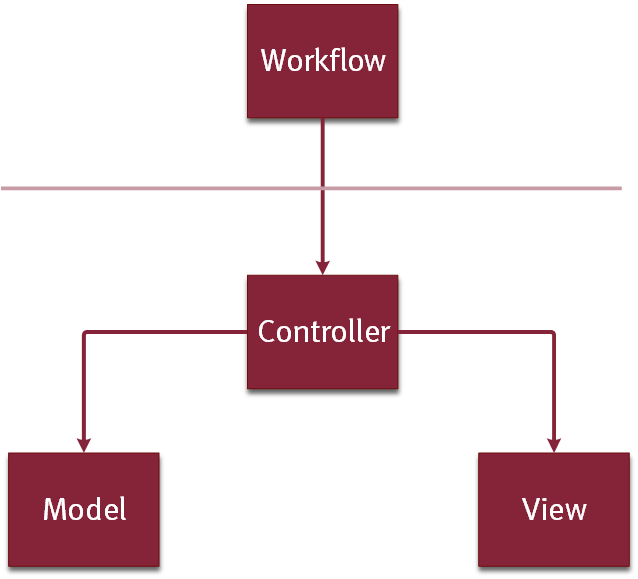
\includegraphics[width = 0.4\linewidth]{Fig/MD2Arch.png}
\caption{Architecture of \MD Models}
\label{fig:MD2Arch}
\end{figure}

All components in \MD are organized in a package structure that represents the aforementioned structure. All documents have to be placed in corresponding packages (views, models, controllers or workflow). For example, all view files are expected to be in the package any.project.package.views. The package has to be defined in each \MD file as follows:
\begin{lstlisting}
package PACKAGE_NAME
\end{lstlisting}
The package name has to be a fully qualified name that reflects the actual folder structure.

\subsubsection{Workflow} 
\label{subsubsec:Workflow}
The workflow layer is an additional abstraction on top of the controller layer. It thereby allows to specify the general course of action of one or more apps with few simple and well understandable model language constructs. Furthermore, this abstract workflow representation is intended to serve as a basis for communication with customers, e.g. for requirements engineering and collaborative app development.

In the workflow file of an MD2 model a workflow can be specified as a (possibly cyclic) directed graph of workflow elements. Workflow elements represent encapsulated functionality which is specified in detail in the controller layer. The workflow layer references the workflow elements from the controller layer to define their interaction.

For this purpose, Workflow elements are linked via events. For each workflow element one or more events can be specified that can be fired. However, at runtime a workflow element can fire only one of these events, i.e. a parallel processing of the workflow is not intended. In addition to the events that can be fired, the workflow element also specifies which workflow element is to be started in response to a fired event using the keyword {\lstinline!start!}.
A workflow element in the workflow layer typically looks as shown in Listing \ref{lst:wfe}.

\begin{lstlisting}[language=MD2, label=lst:wfe, caption=Workflow Elements in the Workflow Layer]
 WorkflowElement NameOfWorkflowElement
 	fires NameOfEventOne {
		start NameOfSubsequentWfeOne
	}
	fires NameOfEventTwo {
		start NameOfSubsequentWfe
	}
\end{lstlisting}

After defining the sequence of workflow elements, the workflow also requires the specification of an app. As shown in Listing \ref{lst:app}, an app consists of its ID, a list of workflow elements that are used in the app and a name that is to be used as app titel. For the scenario where only a single app is modeled, all workflow elements can be listed in the app. However, it is also possible to have unused workflow elements.

\begin{lstlisting}[language=MD2, label=lst:app, caption=App Definition in MD2]
App AppID {
	WorkflowElements {
		WorkflowElementOne,
		WorkflowElementTwo (startable: "Start Workflow Element Two"),
		WorkflowElementThree 
	}
	appName "App Title"
}
\end{lstlisting}

A workflow has one or more entry points, i.e. startable workflow elements. These are marked as {\lstinline!startable!} in the app specification. During code generation this will result in a button within the app that starts the corresponding workflow element. In addition, a string needs to be inserted which is used as label or description for the button.

Finally, the complete workflow specification for one app will be structured as shown in Listing \ref{lst:workflow}. Note that MD2 does not differentiate between different workflows. However, it is possible to implicitly create multiple workflows by using two or more startable workflow elements that start independent, disjunct sequences of workflow elements.

\begin{lstlisting}[language=MD2, label=lst:workflow, caption=Workflow Definition in MD2]
package ProjectName.workflows

WorkflowElement WorkflowElementOne
[...]
WorkflowElement WorkflowElementTwo
[...]
WorkflowElement WorkflowElementThree
[...]

App AppID {
	[...]
}
\end{lstlisting}

\subsubsection{Model} 
\label{subsubsec:Model}

In the model layer the structure of data objects is being described. As model elements Entities and Enums are supported.
\paragraph{Entity}
An entity is indicated by the keyword {\lstinline!entity!} followed by an arbitrary name that identifies it.
\begin{lstlisting}
entity NAME {
<attribute1 ... attribute n>
}
\end{lstlisting}
Each entity may contain an arbitrary number of attributes of the form
\begin{lstlisting}
ATTRIBUTE_NAME: <datatype>[] (<parameters>) {
name STRING
description STRING
}
\end{lstlisting}
The optional square brackets [] indicate a one-to-many relationship. That means that the corresponding object may hold an arbitrary number of values of the given datatype.
Supported complex data types are:
\begin{itemize}
\item{Entity}
\item{Enum}
\end{itemize}
Supported simple data types are:

\begin{itemize}
\item{\lstinline!integer! -- integer}
\item{\lstinline!float! -- float of the form \#.\#}
\item{\lstinline!boolean! -- boolean}
\item{\lstinline!string! -- a string that is embraced by single quotes (') or double quotes (")}
\item{\lstinline!date! -- a date is a string that conforms the following format: \lstinline!YYYY-MM-DD!}
\item{\lstinline!time! -- a time is a string that conforms the following format: \lstinline!hh:mm:ss[(+|-)hh[:mm]]!}
\item{\lstinline!datetime! -- a date time is a string that conforms the following format: \lstinline!YYYY-MM-DDThh:mm:ss [(+|-)hh[:mm]]!}
\end{itemize}

Parameters are optional and will be transformed into implicit validators during the generation process. They have to be specified as a comma-separated list. On default each specified attribute is mandatory. To allow null values the parameter optional can be set. Further supported parameters depend on the used data type and are explained as follows:

\begin{itemize}
\item \lstinline!integer! supports
\subitem \lstinline!max INTEGER! – maximum allowed value of the attribute
\subitem \lstinline!min INTEGER! – minimum allowed value of the attribute
\item \lstinline!float! supports
\subitem \lstinline!max FLOAT! – maximum allowed value of the attribute
\subitem \lstinline!min FLOAT! – minimum allowed value of the attribute
\item \lstinline!string! supports
\subitem \lstinline!maxLength INTEGER! – maximal length of the string value
\subitem \lstinline!minLingth INTEGER! – minimal length of the string value
\end{itemize}

Optionally, attributes can be annotated with a name and a description which are used for the labels and the tooltips in the auto-generation of views. If a tooltip is annotated a question mark will be shown next to the generated input field. If no name is annotated, a standard text for the label will be derived from the attribute's name by transforming the camel case name to natural language. E.g. the implicit label text of the attribute firstName is \enquote{First name}.

Exemplary entity that represents a person:
\begin{lstlisting}
entity Person {
	name: string
	birthdate: date {
		name: "Date of Birth"
		description: "The exact day of birth of this person."
	}
	salary: float (optional, min 8.50, max 1000)
	addresses: Address[]
}
\end{lstlisting}

\paragraph{Enum}
An enumeration is indicated by the keyword \lstinline!enum! followed by an arbitrary name that identifies it. Each enum may contain an arbitrary number of comma-separated strings. Other data types are not supported.
Exemplary enum element to specify weekdays:
\begin{lstlisting}
enum Weekday {
"Mon", "Tue", "Wed", "Thu", "Fri", "Sat", "Sun"
}
\end{lstlisting}


\subsubsection{View} 
\label{subsubsec:View}

\subsubsection{Controller} 
\label{subsubsec:Controller}


\subsection{Deploying a Single App}
\label{subsec:SingleAppDep}

\subsubsection{Backend} 
\label{subsubsec:Backend}

\subsubsection{map.apps} 
\label{subsubsec:mapapps}


\section{Development and Deployment of Multiple Apps}
\label{sec:developAndDeployMultiApps}
% !TeX spellcheck = en_GB
% !TeX program = xelatex
% !TEX root = ../md2-user-handbook.tex

The \MD framework allows to model and generate workflows that involve multiple apps. For this purpose, several apps rather than just one can be specified in the workflow layer. These apps can share the same workflow elements or use different ones as shown in Listing \ref{lst:multipleApps}. Apart from that, the workflow will look as usual, with the sequence of workflow elements being determined via events. Each app is provided with a list of open issues in the start screen. In this list, all events are presented that were fired from another app and are supposed to start a workflow element which belongs to the current app. A user can simply click on a listed issue to continue the workflow in the appropriate workflow element.

\begin{lstlisting}[language=MD2, label=lst:multipleApps, caption=Workflow definition for multiple apps]
package <ProjectName>.workflows

WorkflowElement <WorkflowElementOne>
<...>
WorkflowElement <WorkflowElementTwo>
<...>
WorkflowElement <WorkflowElementThree>
<...>

App <AppID1> {
	<WorkflowElementOne> (startable: STRING),
	<WorkflowElementTwo>
}

App <AppID2> {
	<WorkflowElementOne>,
	<WorkflowElementThree>
}
\end{lstlisting}

The deployment of multiple apps is similar to that of a single app. In this case, however, not just one but all created apps have to be deployed, \eg by setting the corresponding symbolic links as described in  \Cref{subsec:SingleAppDep} for each app.


\section{Additional Features}
% !TeX spellcheck = en_GB
% !TeX program = xelatex
% !TEX root = ../md2-user-handbook.tex

\subsection{Calling RESTful Web Services from an App}
\label{subsec: CallingWebServices}
With the current \MD version it is possible to call RESTful web services that are provided by external applications. To do so, it is necessary to specify the web service's URL and REST method (currently GET, POST, PUT and DELETE are supported), as well as the parameters to be transferred to it. The parameters are represented as <key, value> pairs and can be sent as query parameters and/or via the body of the request. Accordingly, depending on the option expected by the service to be called, the DSL allows the modeler to specify queryparams or bodyparams.

Aside from static values to be set at design time, it is possible to set a parameter to the value of a particular ContentProviderPath, \ie the value of a content provider's field, which is derived at run time. If the value is set statically at design time the data types String, Integer, Float and Boolean are allowed (as they will internally be converted into JSON).

An exemplary web service description based on the DSL as well as the corresponding call of the action is depicted in the following.

\begin{lstlisting}[language=MD2, label=lst:callWSfromWF, caption=Calling a web service from within a workflow]

// Specification of the web service call
externalWebService <externalWebServiceCallOne> {
	url URL
	method (GET | POST | PUT | DELETE)
	queryparams(
		STRING : (INT | STRING | FLOAT | BOOLEAN | <ContentProviderPath>)	
		STRING : (INT | STRING | FLOAT | BOOLEAN | <ContentProviderPath>)
		<...>	
	)
	bodyparams (
		STRING : (INT | STRING | FLOAT | BOOLEAN | <ContentProviderPath>)
		<...>
	)
}

// Specify action to call the web service
action CustomAction <CustomActionOne> {
	call WebServiceCall <externalWebServiceCallOne>
}
	
\end{lstlisting}





\subsection{Controlling a Workflow by calling a RESTful Web Service}
\label{subsec: WorkflowControlThroughWS}
The \MD language offers a possibility to define a RESTful web service according to \Cref{lst:offerWStoSWF}, which will start a certain workflow element. For this purpose for each workflow element marked as \lstinline|invokable| a web service is generated with one endpoint for each invoke definition. 
When an invoke definition is placed within a workflow element of the controller model, the respective workflow element in the workflow model has to be marked as invokable as well. An event description can be added, which will be shown in the list of open issues as the event which was fired last.

\begin{lstlisting}[language=MD2, label=lst:offerWStoSWF, caption=Offer a web service to start a workflow]
invokable at STRING using (POST | PUT) {
	<ContentProviderPath> as ALIAS
	default <ContentProviderPath> = <Value>
	set <ContentProviderPath> to <ContentProvider>
}
\end{lstlisting}
The minimally required invoke definition is simply the keyword \lstinline|invokable|. The standard path where an endpoint is injected is \enquote{/}. If another path should be used this must be defined after the \lstinline|at| keyword. If multiple endpoints are defined, setting the path is mandatory.

The standard REST method used for the RESTful web service endpoint is \lstinline|POST|. However, after the keyword \lstinline|using|, the modeller can choose \lstinline|PUT| instead.
In the body of an invoke definition it can be defined if entities and their attributes should be set during the web service call. Three different possibilities exist for this purpose. In the following they are described in the order of their appearance within \Cref{lst:offerWStoSWF}.

\begin{itemize}
	\item The first type allows attribute values to be set by the web service call. This means that the attribute is transformed to a parameter of the endpoint and is then set to the received value. For the name of the parameter either the name of the attribute is used or an alternative alias can be defined.
	\item If some attributes should always receive the same value regardless of the parameter values, they can be set to a default value using the second type. An example would be a status field which is set to \enquote{issue received} when the workflow is started.
	\item The last type is similar to setting a content provider to an attribute (cf. \Cref{subsubsec:Controller}). Since the language only knows how entities are related to each other, but not their corresponding content providers, this statement is needed for every nested entity.
\end{itemize}

For each entity referenced within the definition an instance of it will be created and persisted. The type of persistence depends on whether the remote connection of the content provider equals the one of the \lstinline|workflowManager|. If they are equal, the web service call and the persistence is handled on the same server, thus the internal Enterprise JavaBeans can be used. Otherwise, the other external backend server needs to be called -- this is however not implemented in the current version of the \MD. It is not only necessary that the URLs of the remote connections are equal, but the objects also need to be identical.
If the body is missing, no entities or attributes are set.



\chapter{Developer's Handbook}

\todo{Short introduction to the dev handbook}
\todo{incl. "whenever the language is changed, it affects the formatter and... , so the dev workflow should always take that into consideration"}

\section{Installation}
% !TeX spellcheck = en_GB
% !TeX program = xelatex
% !TeX root = md2-user-handbook.tex

\subsection{Setting up your \MD model development environment}

The following software is required to enable modelling of \MD models and deployment of generated backends:

\begin{itemize}
\item A current Eclipse IDE with support for Java EE development (e.g. Luna)
\item Using the \href{https://eclipse.org/Xtext/download.html}{Xtext Update Site}, install a current version of the Xtext redistributable
\item From the archive that you obtained, install the \MD features
\item GlassFish 4.+
\end{itemize}

You are ready to go.


\subsection{Setting up a \mapapps development environment}

As a prerequisite, ensure that the following software is installed:

\begin{itemize}
\item map.apps 3.1.0
\item NetBeans EE (e.g. Version 8.0)
\item Apache Tomcat 7.0 with running \mapapps runtime\footnote{For details on their installation, please refer to the \mapapps documentation.}
\end{itemize}

\begin{enumerate}
\item {Basic \mapapps Development Setup} \label{subsec:basic-setup}

\begin{enumerate}
\item Extract the \lstinline|sampleProjRemote| project from the \mapapps distribution and load it in NetBeans. \label{item:extraction}
\item In its \lstinline|pom.xml|,
 set the \lstinline|mapapps.remote.base| directive to the URL where the \mapapps runtime is installed.
\item Right-click the project, select \enquote{Custom} and select \enquote{Goals...} to create a new Maven goal. \todo{Describe configuration}
\item Open the \lstinline|nbactions.xml|. \todo{Describe set property for Jetty port 9090}

\end{enumerate}

\item {Deploy \MD Runtime Bundles}
\begin{enumerate}
\item Copy the \MD runtime bundles into the \texttt{bundles/} directory of the project:
	\begin{quotation}
		 \texttt{md2\_formcontrols}
		 
		 \texttt{md2\_local\_store}
		 
		 \texttt{md2\_location\_service}
		 
		 \texttt{md2\_runtime}
		 
		 \texttt{md2\_store}
		 
		 \texttt{onlinestatus}
	\end{quotation}

\item Copy a generated \MD App into the project or use a symlink to reference Apps from another location (see \Cref{subsec:link-apps}).
\end{enumerate}


\end{enumerate}

\section{DSL Semantics}
% !TeX spellcheck = en_GB
% !TeX program = xelatex
% !TeX root = ../md2-user-handbook.tex

The \MD framework is intended to provide a cross platform solution, i.e. to generate apps not only for map.apps but also other platforms. For this purpose, this section delivers an overview about the semantics of the DSL, e.g. the different patterns targeted or forms of communication that are implicated by certain model constructs. This will enable future developers to generate apps for other platforms which provide the same functionality as the apps currently generated for map.apps.

First of all, the MVC pattern with additional workflow layer used in the DSL should also be represented in the generated code.

\paragraph{Workflow Layer}
The workflow layer defines different apps and their workflow elements. Since workflows bundle specific functionality, each app can be seen as a user role, and the assigned workflow elements represent the role's permissions. However, a sphisticated user or role management is not implemented for the \MD framework.

Every app is supposed to be given a start screen which contains buttons for workflow elements that can be started from the app as well as a list of open issues that can be continued by the app. The belongingness of workflow elements to apps should be represented in a map in the backend, which connects workflow elements to their apps. This is for example important for the determination of open issues which are allowed to be continued from a specific app.

Similar to that, the backend needs to know the sequence of workflow elements, i.e. which workflow elements are to be started after which event and when to end the workflow. Note that two workflow elements can fire the same event and start different workflow elements. Thus, the backend also needs to know which event/workflow element combination initializes the start of a specific new workflow element.

However, if a workflow element fires an event which starts a new workflow element within the same app, this should be handled by the app-specific EventHandler, i.e. no backend communication is required. This is important if future developments are supposed to allow for temporary off-line usage of apps. Thus, the backend handles the start of new workflows \textit{across} apps (currently implemented as EventHandlerWS) and the app-secific event handler handles the start of new workflow elements \textit{within} apps.

When a workflow element is started across apps, it will appear in the list of open issues of all apps that have the respective workflow element assigned.

\paragraph{Model Layer}
The model is a quite thin layer in the overall architecture, the only components contained are entities and enumerations. In order to access core data functionality, a data model has to be setup that defines the database to be accessed later on by the content providers. This database is currently located in the backend and should therefore be accessible by apps from all platforms. 

\paragraph{Controller Layer}
The major and biggest layer in this architecture is the controller layer and has the most important role in connecting the view with the model and vice versa. It consists of several workflow elements, each being an independent controller. The default process chain of a workflow element should be used as starting process chain. Likewise the first view from this process chain should be used as start view for the workflow element. Each workflow element (i.e. each controller) requires its own initialization, e.g. mappings of content to views. The required actions for initializations can be found in the onInit block in a workflow element. When a workflow element fires a workflow event, it should be terminated and the control handed to the app-specific EventHandler or the backend as described for the workflow layer. 

Within the body of workflow elements, the controller behavior can be defined using actions and ProcessChains. ProcessChains will be converted to actions in the preprocessor, and therefore do not require a generator for different platforms.

ContentProvider in the controller layer are used for data provision. A webservice-based communication to the backend is required for every platform in order to store and request the data.

\paragraph{View Layer}

The view layer has not been changed during the course of this project seminar. View elements should be implemented with the functionality described in Chapter \ref{cha:modelersHandbook}. 

\section{map.apps Implementation}
% !TEX root = ../md2-user-handbook.tex
% !TeX spellcheck = en_GB
% !TeX program = xelatex

The current implementation of the \MD framework generates web-based apps for a framework called map.apps, which is mainly based on JavaScript. Code generation of Android and iOS apps are also targeted, but not fully implemented yet.

The generated code for \mapapps can be subdivided into three parts: static \mapapps code, dynamically generated \mapapps code and a backend. The static \mapapps code contains the part of the code which does not depend on the models created in the \MD DSL. Since it is static, it does not need to be generated, but is required for the overall functionality of the generated apps. The dynamically generated part is completely dependent on the model. The backend is implemented in Java and contains static as well as dynamic code. However, it is completely generated. The backend provides a server which offers functionality such as data storage and communication accross apps.

Each of these three parts of the code is described in detail in the following.

% start of section for static map.apps implementation

\subsection{Static \mapapps Implementation}

The static \mapapps code is split into several bundles, which are then used by the generated \mapapps code. These bundles are located at \lstinline!src/main/js/bundles!\todo{Keywords nur highlighten wenn freigestellt} and are explained in the following subsections.

\subsubsection{Form controls}

The form controls are defined within the bundle \lstinline!md2_formcontrols!. It uses and extends the existing \mapapps bundle \lstinline|dataform| with additional form elements, which can be used in \MD. Each factory defined within the bundle of \MD, specifies how a JavaScript-object can be transformed to a data form widget. To define an own dataform or to understand the concepts of a dataform component the \href{http://developernetwork.conterra.de/documentation/31/developers/dataform}{\mapapps documentation} will be helpful.

\begin{description}
	\item[DateTimeBoxFactory] Defines a form control for the component \lstinline|DateTimeInput|, which is identified by the keyword \lstinline|datetimebox|. The widget shows a view element showing the time and the date of a \lstinline|datetime| value.
	\item[GridPanelFactory] Defines a form control for the component \lstinline|GridLayoutPane|, which is identified by the keywords \lstinline|md2gridpanel| and \lstinline|gridpanel|. The widget enables to structure multiple view elements in a grid.
	\item[ImageFactory] Defines a form control for the component \lstinline|Image|, which is identified by the keyword \lstinline|image|. The widget is able to display a static image within your app.
	\item[SpacerFactory] Defines a form control for the component \lstinline|Spacer|, which is identified by the keyword \lstinline|spacer|. A spacer defines some white space between some components or within the grid of a \lstinline|GridLayoutPane|.
	\item[StackContainerFactory] Defines a form control for the component \lstinline|AlternativesPane|, which is identified by the keyword \lstinline|stackcontainer|. This widget encapsulates the stackcontainer within \href{http://dojotoolkit.org/reference-guide/1.10/dijit/layout/StackContainer.html}{\lstinline|dijit/layout/StackContainer|}. It provides a view elements which has multiple views, but shows only one, similar to a book or a slide show. The user can navigate between them using specific keys. 
	\item[TextOutputFactory] Defines a form control for the component \lstinline|Label|, which is identified by the keyword \lstinline|textoutput|. This widget enables to display uneditable text.
	\item[TooltipFactory] Defines a form control for the component \lstinline|Tooltip|, which is identified by the keyword \lstinline|tooltipicon|. This widget offers a tooltip behind a question mark icon.
	\item[UploadImageOutputFactory] Defines a form control for the component \lstinline|UploadedImageOutput|, which is identified by the keyword \lstinline|uploadimageoutput|. The widget is able to display an image within your app, which is uploaded/specified by the user.
\end{description}

\subsubsection{List of open issues}
\label{sec:listOfOpenIssues}

The \lstinline!md2_list_of_open_issues! comprises all code necessary for displaying the list of open issues within the app. This list shows all workflow instances, whose state is at a workflow element, which belongs to the current app. Currently supported data listed in this widget are the guid of the workflow instance, the workflow element name and the last fired event. 
The list is included as \lstinline!dijit\_Widget! and is listed as a \texttt{Tool} within the app.json under the bundle specifications of \lstinline!toolset!. In the \lstinline!ListOfOpenIssuesController! a \lstinline!DataView! is created, which uses the workflow store as a \lstinline!DataViewModel!. The workflow store is described in \cref{workflow_store}.
In addition to just displaying the workflow instances it is possible to start the workflow element through clicking on the respective entry. Therefore the \lstinline!ListOfOpenIssuesController! handles the event \lstinline!onClicked! and calls the function \lstinline!startWorkflow! of the respective \lstinline!MD2MainWidget!.

\subsubsection{Local store}

The local store within the bundle \lstinline|md2_local_store| is one of three stores used in the context of \mapapps within \MD. This store implements some of the guidelines from the \lstinline|dojo/Store| interface, which means, that it offers the methods \lstinline|query|, \lstinline|get|, \lstinline|put|, \lstinline|add|, and \lstinline|remove|.
The local store can be used by a content provider (set to local within the controller model). This store saves all data as cookies in the browser. Thus the store is not meant for consistent data storage.

\subsubsection{Location service}

\subsubsection{Runtime}\todo{Add descriptions of folders: 
contentprovider, 
datamapper, 
datatypes, 
entities, 
events, 
handler, 
legacy, 
resources, 
templates, 
util, 
validators, 
view}

\paragraph{MD2MainWidget}
Each workflow element (see \ref{sec:developAndDeployMultiApps}) has its own instance of a \MD main widget. This is specified in the respective controller of the workflow element bundle inside the app. That is, the \lstinline!manifest.json! of the workflow element bundle references an \lstinline!_md2AppWidget! for its controller. Once the controller is activated (i.e. the \lstinline!activate! function is called), the respective \MD main widget instance is built. This \MD main widget is implemented in the file \lstinline!MD2MainWidget!, which serves as the basic starting point to start a workflow. Thus, it provides methods to start a workflow element. There are different ways a workflow can be started. One way is to start it directly from the map.apps tool bar. Another way is to start a workflow from the list of open issues (see section \ref{sec:listOfOpenIssues}). Figure~\ref{fig:InitMD2MainWidget} depicts this initialization process.

\begin{figure}
\centering
\begin{tikzpicture}[
	redbox/.style = {rectangle, fill=ercisred, text =white, draw=none, text centered, drop shadow},
	arrowlbl/.style = {pos=.5, black},
	>=stealth
]

\draw (-3.5,-2.25) rectangle (1.2,-0.5);
\draw [fill=gray!20!white] (-3.5,-0.9) rectangle (-0.7,-0.5) node[pos=.5] {\small{List of open issues}};
\draw [redbox] (-3.3,-2) rectangle (1,-1) node[pos=.5] {OpenIssueListController};

\draw [->, thick, ercisred] (1,-1.1) -- (4.2,-1.1) node[above, arrowlbl] {\lstinline!startWorkflow!} -- (4.2,0.4) -- (6.5,0.4);

\draw [->, thick, ercisred] (1,-1.9) -- node[above, arrowlbl] {\lstinline!getMD2MainWidget!} (6,-1.9);

\node[draw] (tool) at (-1.25, -3) {\small{\textit{map.apps tool}}};
\draw [->, thick, ercisred] (tool) -- (5.35,-3) node[above, arrowlbl] {\lstinline!startWorkflowFromTool!} -- (5.35,0.2) -- (6.5,0.2);

\draw [->, thick, ercisred] (-2.9,1) -- node[above, arrowlbl] {\lstinline!load!} (-1.9,1);

\node [above] at (-0.9,0.5) {\lstinline!activate!};
\draw [->, thick, ercisred] (-1.8,1) -- (-1.8,0.5) -- (0,0.5);
\draw [fill=gray!20!white](-1.9,1.1) rectangle (-0.8,1.5) node[pos=.5] {\small{WfE}};
\draw (-1.9,-0.25) rectangle (2.25,1.5);
\draw [redbox] (0,0) rectangle (2,1) node[pos=.5] {Controller};

\draw [->, thick, ercisred] (2,0.65) -- node[above, arrowlbl] {\lstinline!build!} (6.5,0.65);

\draw [fill=gray!20!white] (5.5,1.1) rectangle (8,1.5) node[pos=.5] {\small{MD2Runtime}};
\draw (5.5,-2.25) rectangle (11.25,1.5);
\draw [redbox] (6.5,0) rectangle (11,1) node[pos=.5] {MD2MainWidget};
%\node [rotate=270] at (10.7,0.35) {\small{startWorkflow}};
%\draw [->, thick, ercisred] (10,0.8) -- (10.5,0.8) -- (10.5,0.2) -- (10,0.2);

\draw [->, thick, ercisred] (7,0) -- node[right, arrowlbl] {\lstinline!register!} (7,-1);

\draw [redbox] (6,-2) rectangle (11,-1) node[pos=.5] {WorkflowStateHandler};

\end{tikzpicture}
\caption{Initialization of the \MD main widget in order to start a workflow}
\label{fig:InitMD2MainWidget}
\end{figure}

\paragraph{Workflow}\todo{Erlaeuterung der transactionID im WorkflowStateHandler + Erlaeuterung vom WorkflowStateTransaction.js fehlt noch...}
For each started workflow instance an unique ID is generated and assigned to that instance. This is done in the method \lstinline!startWorfklow! of the \lstinline!MD2MainWidget!. A global \lstinline!WorkflowStateHandler! provides methods to set and get the currently active workflow instance ID. This information is needed to suspend a workflow and to resume that workflow at a later time.

\paragraph{Actions}
Each action that is defined in the \MD DSL must also exist in the \MD runtime bundle in map.apps to be used. Individual actions are stored in the subfolder \lstinline!simpleactions!. Moreover, an \lstinline!ActionFactory! must provide a simple method that returns an instance of the respective action (e.g., \lstinline!getLocationAction! for the \lstinline!LocationAction!). All actions provide a method \lstinline!execute! that implements the action. An individual constructor allows to initialize the action, e.g., setting the city's name for a \lstinline!LocationAction!. The \lstinline!ActionFactory! is instanced in the method \lstinline!build! of the \lstinline!MD2MainWidget! (see figure~\ref{fig:InitMD2MainWidget}). Thus, every workflow element can access and use this factory.

\subsubsection{Store}

\subsubsection{Workflow store} \label{workflow_store}

% end of section for static map.apps implementation

\subsection{Dynamic map.apps implementation} \todo{Maybe join this with the \enquote{map.apps Generator} section}

\subsection{Backend} \todo{as part of map.apps? I'd suggest to move this into its own section -- Jan}


\section{map.apps Generator}
% !TeX spellcheck = en_GB
% !TeX program = xelatex
% !TeX root = ../md2-user-handbook.tex

\todo{empty @ALL [why is this chapter after the map.apps Implementation?]}

%%%%%%%%%%%%%%%%%%%%%%%%%%%%%%%%%%%%%%%%%%%%%%%%%%%%%%%%%%%%%%%%
%% appendix

\clearpage
\appendix
\pagenumbering{Roman}		%% roman page numbers for the appendix
%\input{90-Appendix}

\chapter{Sample Workflow}
% !TeX spellcheck = en_GB
% !TeX program = xelatex
% !TeX root = md2-user-handbook.tex






%% Stop section "numbering" after appendix

\setcounter{secnumdepth}{0}

%%%%%%%%%%%%%%%%%%%%%%%%%%%%%%%%%%%%%%%%%%%%%%%%%%%%%%%%%%%%%%%%
%% lists of figures and tables

%\clearpage
%\listoffigures
%\listoftables

%%%%%%%%%%%%%%%%%%%%%%%%%%%%%%%%%%%%%%%%%%%%%%%%%%%%%%%%%%%%%%%%
%% Define Abbreviations
%\clearpage
%\section{List of Acronyms}
%\begin{acronym}
%\acro{AACS}{Advanced Access Content System}
%\acro{XOR}{exclusive or}
%\end{acronym}

%\clearpage
%%%%%%%%%%%%%%%%%%%%%%%%%%%%%%%%%%%%%%%%%%%%%%%%%%%%%%%%%%%%%%%%
%% bibliography (if needed)

%\nocite{*}
%\bibliographystyle{plain}
%\bibliography{lit}

%\printbibliography[heading=bibintoc] % biblatex
\end{document}